\documentclass[a4paper,fleqn]{cas-sc}
% High-level Commands
\newcommand{\version}{v1/}
\newcommand{\eg}{\textit{e.g.}}

% Math Commands
\newcommand{\dispx}{u_{x_{1:t}}}
\newcommand{\dispy}{u_{y_{1:t}}}
\newcommand{\avgstress}{\bar{\sigma}_{1:t}}
\newcommand{\avgstrain}{\bar{\epsilon}_{1:t}}

\usepackage[authoryear,longnamesfirst]{natbib}
%\RequirePackage{cas-common}

%%%Author macros
\def\tsc#1{\csdef{#1}{\textsc{\lowercase{#1}}\xspace}}
\tsc{WGM}
\tsc{QE}

% Uncomment and use as if needed
%\newtheorem{theorem}{Theorem}
%\newtheorem{lemma}[theorem]{Lemma}
%\newdefinition{rmk}{Remark}
%\newproof{pf}{Proof}
%\newproof{pot}{Proof of Theorem \ref{thm}}

\begin{document}
\let\WriteBookmarks\relax
\def\floatpagepagefraction{1}
\def\textpagefraction{.001}

% Short title
\shorttitle{Cooperative Data-driven Modeling}    

% Short author
%\shortauthors{<short author list for running head>}  

% Main title of the paper
\title[mode=title]{Cooperative Data-driven Modeling}  

% Title footnote mark
% eg: \tnotemark[1]
%\tnotemark[1] 

% Title footnote 1.
% eg: \tnotetext[1]{Title footnote text}
%\tnotetext[1]{Title footnote text} 

% First author
%
% Options: Use if required
% eg: \author[1,3]{Author Name}[type=editor,
%       style=chinese,
%       auid=000,
%       bioid=1,
%       prefix=Sir,
%       orcid=0000-0000-0000-0000,
%       facebook=<facebook id>,
%       twitter=<twitter id>,
%       linkedin=<linkedin id>,
%       gplus=<gplus id>]

\author[1]{A}

% Corresponding author indication

% Footnote of the first author
%\fnmark[<footnote mark no>]

% Email id of the first author
%\ead{<email address>}

% URL of the first author
%\ead[url]{<URL>}

% Credit authorship
% eg: \credit{Conceptualization of this study, Methodology, Software}
%\credit{<Credit authorship details>}

% Address/affiliation
\affiliation[1]{organization={Delft University of Technology},
            addressline={}, 
            city={},
%          citysep={}, % Uncomment if no comma needed between city and postcode
            postcode={}, 
            state={},
            country={}}


\author[2]{B}
% Footnote of the second author
%\fnmark[2]

% Email id of the second author
%\ead{}

% URL of the second author
%\ead[url]{}

% Credit authorship
%\credit{}

% Address/affiliation
\affiliation[2]{organization={Delft University of Technology},
            addressline={}, 
            city={},
%          citysep={}, % Uncomment if no comma needed between city and postcode
            postcode={}, 
            state={},
            country={}}



\author[3]{C}
% Footnote of the third author
%\fnmark[3]

%Email id of the third author
\ead{miguel_bessa@brown.edu}

% URL of the third author
%\ead[url]{}

% Credit authorship
%\credit{}

% Address/affiliation
\affiliation[3]{organization={Brown University},
            addressline={}, 
            city={},
%          citysep={}, % Uncomment if no comma needed between city and postcode
            postcode={}, 
            state={},
            country={}}

\cormark[1]
\cortext[1]{Corresponding author}

% Footnote text
%\fntext[3]{}

% For a title note without a number/mark
%\nonumnote{}

% Here goes the abstract
\begin{abstract}
Abstract
\end{abstract}

% Use if graphical abstract is present
%\begin{graphicalabstract}
%\includegraphics{}
%\end{graphicalabstract}

% Research highlights
\begin{highlights}
\item 
\item 
\item 
\end{highlights}

% Keywords
% Each keyword is seperated by \sep
\begin{keywords}
 \sep data-driven modeling \sep continual learning \sep transfer learning \sep plasticity
\end{keywords}

\maketitle

% Numbered list
% Use the style of numbering in square brackets.
% If nothing is used, default style will be taken.
%\begin{enumerate}[a)]
%\item 
%\item 
%\item 
%\end{enumerate}  

% Unnumbered list
%\begin{itemize}
%\item 
%\item 
%\item 
%\end{itemize}  

% Description list
%\begin{description}
%\item[]
%\item[] 
%\item[] 
%\end{description}  

% Figure
%\begin{figure}[<options>]
%	\centering
%		\includegraphics[<options>]{}
%	  \caption{}\label{fig1}
%\end{figure}


%\begin{table}[<options>]
%\caption{}\label{tbl1}
%\begin{tabular*}{\tblwidth}{@{}LL@{}}
%\toprule
%  &  \\ % Table header row
%\midrule
% & \\
% & \\
% & \\
% & \\
%\bottomrule
%\end{tabular*}
%\end{table}

% Main text
\section{Introduction}\label{sec:intro}
  \section{Introduction}
\begin{frame}{Computational Solid Mechanics}
  \begin{minipage}{0.5\textwidth}
    \only<1>{
    \begin{block}{\color{White} Solid Mechanics}
      \begin{itemize}
        \item \color{Black} Relate deformation with internal force development
        \item $\boldsymbol{\nabla} \cdot \mathbf{P}= 0$ with \color{White} $\mathbf{P}=\mathcal{C}(\mathbf{F})$
      \end{itemize}
    \end{block}
    }
    \only<2>{
    \centering
    \includegraphics[width=0.85\textwidth]{Figures/intro/link}
    }
  \end{minipage}%
  \begin{minipage}{0.5\textwidth}
    \only<1>{
    \centering
    \includegraphics[width=0.85\textwidth]{Figures/intro/link}
    }
    \only<2>{
    \begin{block}{\color{White}Finite Element Method}
      \begin{itemize}
        \item General PDE solving method
        \item Discretize the domain 
        \item Weakly satisfy the PDE at selected points
      \end{itemize}
    \end{block}
  }
  \end{minipage}
\end{frame}

\begin{frame}{Composite Modeling}
  \begin{minipage}{0.5\textwidth}
  \only<1>{
    \centering
    \includegraphics[width=2\textwidth]{Figures/intro/scales}
    }
    \only<2>{
    \begin{block}{\color{White}FE$^2$}
      \begin{itemize}
        \item Representative Volume Element (RVE)
        \item Solve for RVE and average the response
        \item Repeat for every selected point
      \end{itemize}
    \end{block}
  }

  \only<3,4>{
  \begin{block}{\color{White}FE$^2$-Bottleneck}
      \begin{itemize}
        \item Micro-scale problem solution
        \item Repeating for every selected point
        \item Highly non-linear behaviour 
      \end{itemize}
    \end{block}
  }
  \end{minipage}%
  \begin{minipage}{0.5\textwidth}
  \only<2>{
    \centering
    \includegraphics[width=0.9\textwidth]{Figures/intro/FE2-CONV}
  }
  \only<3,4>{
    \centering
    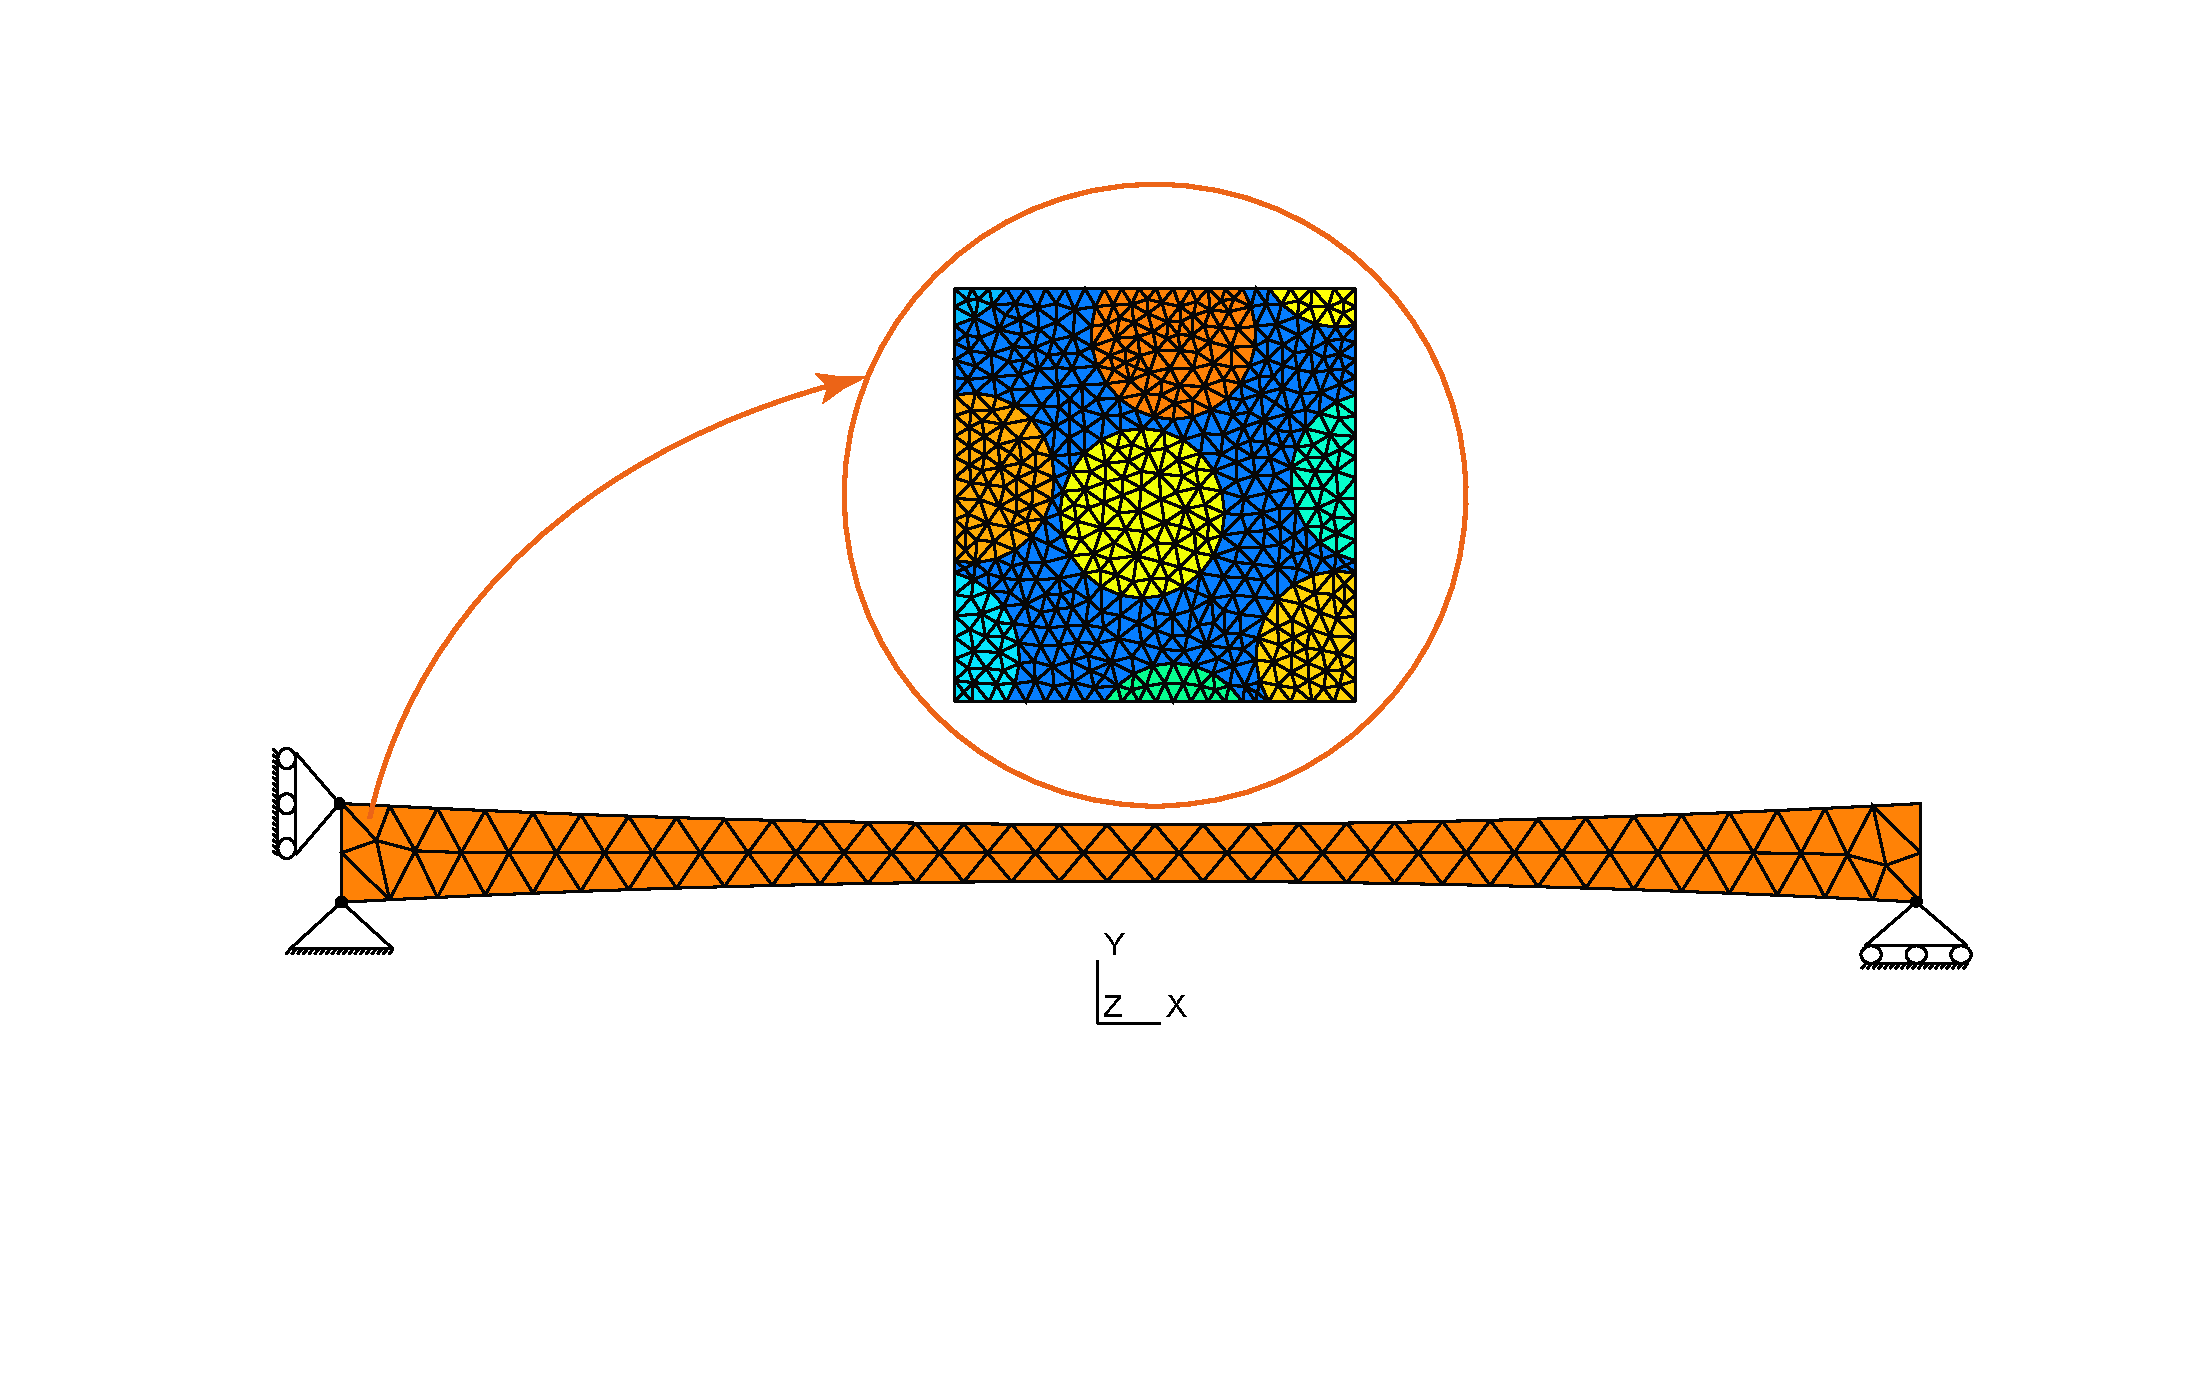
\includegraphics[width=\textwidth]{Figures/intro/bone}
  }
  \end{minipage}
  \only<4>{
    \centering
    \color{Pink} We need multiple of these simulations for real world applications!
  }
\end{frame}


\section{Continual learning}\label{sec:cl}

\subsection{Methods overview}\label{subsec:overview}

\section{Proposed method (CDDM)}\label{sec:method}

\section{Numerical experiments}\label{sec:numerical_exp}

\subsection{Data generation}\label{subsec:data}

\subsection{Results}\label{subsec:results}

\section{Discussion}\label{sec:discussion}

\section{Conclusion}\label{sec:conclusion}


%% \appendix

% To print the credit authorship contribution details
%\printcredits

%% Loading bibliography style file
%\bibliographystyle{model1-num-names}
\bibliographystyle{cas-model2-names}

% Loading bibliography database
\bibliography{/home/taylanot/Dropbox/archive_bib/aleksandr_colab.bib}

% Biography
%\bio{}
% Here goes the biography details.
%\endbio

%\bio{pic1}
% Here goes the biography details.
%\endbio

\end{document}

